
\section{Introduction}
\label{sec:introduction}
%%% General intro
\PARstart{T}{he} exponential improvement in computing performance and the availability of large amounts of data are boosting the use of Artificial Intelligent (AI) applications in our daily lives. Among the various algorithms developed over the years, neural networks (NNs) have demonstrated remarkable performance in a variety of image, video, audio, and text analytics tasks \cite{schmidhuber2015deep,Taigman_2014_CVPR}. Historically, ANNs can be classified into three different generations \cite{Design_Exploration_SbS_Trans20}: the first one is represented by the classical McCulloch and Pitts neuron model using discrete binary values as outputs; the second one is represented by more complex architectures as Multi-Layer Perceptrons and Convolutional Neural Networks (CNN) using continuous activation functions; while the third generation is represented by Spiking Neural Networks using spikes as means for information exchange between groups of neurons. Although the AI research is currently dominated by Deep Neural Networks (DNN) from the second generation, nowadays the SNNs belonging to the third generation are receiving considerable attention \cite{Spinnaker_Trans13,ernst2007efficient,Design_Exploration_SbS_Trans20, SNN_Survey_Trans19} due to their advantages in terms of robustness and the potential to achieve a power efficiency closer to that of the human brain (see section~\ref{sec:sbs} for more details).

%%% SbS intro
Among the family of SNNs, the SbS neural network \cite{ernst2007efficient} is inspired by the natural information processing of the mammalian brain, being a biologically plausible approach although with less complexity than other SNNs. The SbS model differs fundamentally from conventional ANNs since (a) the building block of the network are inference populations (IP) which are an optimized generative representation with non-negative values, (b) time progresses from one spike to the next, preserving the property of stochastically firing neurons, and (c) a network has only a small number of parameters, which is an advantageous noise-robust stochastic version of Non-Negative Matrix Factorization (NNMF). In regard to biological realism and computational effort to simulate neural networks, these properties place the SbS network in between non-spiking NN and stochastically spiking NN \cite{rotermund2019Backpropagation}.


%%%%%%% Problem statement
Although SbS networks provide numerous advantages over traditional ANNs and CNNs, deep SbS networks are highly compute and data intensive, representing a challenge for efficient deployment in resource-limited devices. %As an emerging SNN algorithm, most SbS models use floating-point numerical representation, which imposes high complexity of the required circuits for the floating-point operations. Model quantization has the potential to improve computational performance; however, this solution is often accompanied by quantization-aware training methods that, in some cases, are problematic or even inaccessible, particularly in deep SNN algorithms\cite{zhang2018survey}. 
As an alternative, based on the relaxed need for fully precise or deterministic computation of neural networks, approximate computing techniques allow substantial enhancement in processing efficiency with moderated accuracy degradation. Some research papers have shown the feasibility of applying approximate computing to the inference stage of neural networks \cite{lotrivc2012applicability, sarwar2016multiplier, mrazek2016design, du2014leveraging}. Such techniques usually demonstrated small inference accuracy degradation, but significant enhancement in computational performance, resource utilization, and energy consumption. Hence, by taking advantage of the intrinsic error-tolerance of neural networks, approximate computing is positioned as a promising approach for inference on resource-limited devices.

%%%%%%% Contributions
In this paper, we accelerate SbS neural networks with a dot-product hardware design with dynamic approximation scheme based on truncation, this approach leverages the intrinsic error-tolerance of neural networks. For quality configurability, we parameterized the mantissa bit-width of the floating-point synaptic-weight vector. As a design parameter, the mantissa bit-width provides a tunable knob to trade-off between efficiency and quality of result (QoR)\cite{park2009dynamic, han2013approximate}. Since the lower-order bits have smaller significance than the higher-order bits, removing them may have only a minor impact on QoR \cite{gupta2011impact, mittal2016survey}. Further on, we can remove completely the mantissa bits in order to use only the exponent of a floating-point representation. Therefore, the worst-case quality configuration becomes a logarithmic representation, which consequently leads to meaningful architectural-level optimizations using only adders and shifters for dot-product approximation in hardware (see \fig{fig:dot_product_unit}). Moreover, since approximations and noise have qualitatively the same effect\cite{venkataramani2015approximate}, we introduce a noise tolerance plot to intuitively visualize the impact of approximation processing on the neural network accuracy.

\begin{figure}
	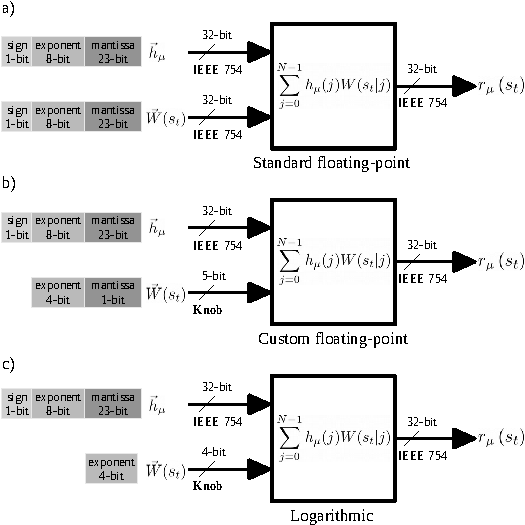
\includegraphics[width=\columnwidth]{../figures/dot-product_unit.pdf}
	\caption{Dot-product hardware module with (a) standard floating-point computation, (b) hybrid custom floating-point approximation, and (c) hybrid logarithmic approximation.}
	\label{fig:dot_product_unit}
\end{figure}

Our main contributions are as follows:

\begin{itemize}
	\item We develop a hardware component for dot-product approximation. To perform the sum of pairwise products of two vectors, this hardware module has the following three design features: (1) the pairwise product is approximated by adding integer exponents, and the sum of products is done by accumulating denormalized integer products, which increases computational throughput; (2) the synaptic weight vector uses either reduced custom floating-point or logarithmic representation, which reduces memory footprint; and (3) the neuron vector uses either standard or custom floating-point representation, which preserves QoR and overall inference accuracy.
	\item We address a design exploration with the proposed dot-product approximation using synaptic weight vector with 1-bit mantissa as well as completely truncated. We evaluate inference latency, accuracy degradation, resource utilization and power dissipation. Experimental results demonstrate $20.49\times$ latency enhancement versus embedded CPU (ARM Cortex-A9 at 666MHz), and less than $0.5\%$ of accuracy degradation on MNIST classification task.
	\item We propose a noise tolerance plot as quality monitor, which serves as an intuitive visual model to provide insights into the accuracy degradation of SbS networks under approximate processing effects.
	\item Our proposed design for dot-product approximation is adaptable as a building block for other error-resilient applications (e.g., image/video processing)
\end{itemize}


The rest of the paper is organized as follows. Section~\ref{sec:related_work} covers the related work; Section~\ref{sec:background} introduces the background to SbS networks; Section~\ref{sec:system_design} describes the system design and the approximate dot-product hardware module; Section~\ref{sec:experimental_results} presents the experimental results thorough a design exploration flow; Section~\ref{sec:conclusions} concludes the paper.


To promote the research on SbS networks, our design exploration framework is made available to the public as an open-source project at http://www.ids.uni-bremen.de/sbs-framework.html

